\chapter{Implementation}\label{ch:experiments}

This chapter describes how the design of \cref{ch:methods} was realised:
the representative system used for development, each implementation
stage with its code artefacts, and the concrete measurements obtained at
each stage.

\section{Representative System: CPSCore}\label{sec:cpscoreintro}

The pipeline was developed and validated on \emph{CPSCore}
\cite{theile:cpscore}, an open-source modular \Cpp\ framework for
cyber-physical systems originally built for the uavAP autopilot project.
It was chosen for three reasons: it is freely available, it uses a real
event-driven publish-subscribe architecture, and its test suite (1,425
assertions across 61 test cases) provides a ground truth for
behavioural verification.

\subsection{Scale and Dispatch Characteristics}\label{sec:cpscore-scale}

CPSCore is a small codebase: 154 source and header files, roughly
13,000 lines (3,800 in \texttt{.cpp} files, 9,200 in headers). It relies
heavily on \texttt{template}-based static polymorphism ($\approx$470
occurrences) and declares only 32 \texttt{virtual} method signatures
across 12 files, all confined to a single module (Utilities:
\texttt{INetworkLayer}, \texttt{ITransportLayer}, \texttt{IPublisherImpl},
\texttt{IScheduler}) or to per-module configuration boundaries
(\texttt{IConfigurableObject}, \texttt{IRunnableObject}). No
cross-module call resolves through a virtual table; inter-module calls
go through concrete class references or \texttt{boost::signals2} slot
connections.

This has a direct consequence for H1 (\cref{sec:h1-results}): since every
cross-module target is statically determinate, the static call graph is
reachability-complete with respect to the trace, and every edge the
trace discovers is already present statically (C3~$\subseteq$~C2). A
codebase with cross-module virtual dispatch or dynamic plugin loading
would likely break this containment and make the dynamic evidence
genuinely additive; CPSCore does not exhibit that property, which is
why C4~$=$~C2 on these scenarios (\cref{sec:h1-c4c2}).

\subsection{CPSCore Architecture}

CPSCore is organised into five modules: \textbf{Aggregation} (component
wiring and lifecycle), \textbf{Configuration} (property mapping),
\textbf{Synchronization} (run-stage scheduling), \textbf{Logging}
(\texttt{CPSLogger}, \texttt{RAIILogStream}), and \textbf{Utilities}
(schedulers, data presentation, signal handling, \ac{IPC}, IDC).
External dependencies are Eigen3, Boost.System, \texttt{cpp\_redis}/tacopie,
and Catch2.

\subsection{Publish-Subscribe via IDC and Redis}\label{sec:idc}

Inter-component communication runs through the \ac{IDC} abstraction
layer, whose two operations (\texttt{subscribeOnPacket},
\texttt{sendPacket}) delegate to a pluggable \texttt{INetworkLayer}. The
default \texttt{RedisNetworkLayer} maps channel identifiers to
\texttt{RedisSubscriber}/\texttt{RedisPublisher} objects backed by
\texttt{cpp\_redis}, wired through a \texttt{boost::signals2} slot
(\texttt{onPacket\_.connect(slot)}) that fires when a Redis message
arrives -- the concrete instance of the call-site blind spot that
\cref{sec:macro-resolution} resolves.

\section{Stage 1: Static Analysis and Graph Population}\label{sec:static-impl}

\subsection{Renaissance to Neo4j}

CPSCore's source tree was analysed by Renaissance, which resolves the
full \ac{AST} (template instantiations, overload candidates, macro
expansions) and emits the property graph schema in
\cref{tab:node-types,tab:edge-types}: 11 node labels and 11 relationship
types, all from static analysis, populating a graph of 67,104 nodes.
Runtime traces are processed separately into a sequence table and
combined with the static edge set only at evaluation time
(\cref{sec:combine-scope}).

\section{Stage 2: Code Graph Query}\label{sec:query-impl}

\subsection{Schema Introspection Skill}

The \texttt{get-neo4j-schema} skill runs three Cypher statements against
the live graph to produce a machine-readable schema summary for
downstream skills:

\begin{minted}{cypher}
-- Node labels and properties
CALL db.schema.nodeTypeProperties()
YIELD nodeType, propertyName, propertyTypes
RETURN nodeType, propertyName, propertyTypes;

-- Relationship types and properties
CALL db.schema.relTypeProperties()
YIELD relType, propertyName, propertyTypes
RETURN relType, propertyName, propertyTypes;

-- Relationship signatures (which label pairs each edge connects)
MATCH (s)-[r]->(t)
RETURN DISTINCT labels(s) AS fromLabels,
                type(r)   AS relType,
                labels(t) AS toLabels;
\end{minted}

\subsection{Scenario-Scoped Query}\label{sec:scenario-query-impl}

For a given scenario, \texttt{text-to-cypher} translates the scenario
description into a schema-aware Cypher query and \texttt{cypher-to-output}
executes it against the live graph, returning the scenario-scoped
subgraph consumed by Stage~3. For S1 (``Using agent skills, show me
Synchronization calling into Aggregation and Logging''):

\begin{minted}{cypher}
// scoped to S1: Synchronization / Aggregation / Logging
MATCH (caller)-[:CppCalls]->(callee)
WHERE (caller.name CONTAINS '/src/Synchronization/'
    OR caller.name CONTAINS '/include/cpsCore/Synchronization/')
  AND (callee.name CONTAINS '/Aggregation/' OR callee.name CONTAINS '/Logging/')
RETURN DISTINCT
    caller.name AS callerName, caller.symbol AS callerSymbol,
    callee.name AS calleeName, callee.symbol AS calleeSymbol
\end{minted}

Before this query runs, the running example edge
\texttt{SynchronizedRunner.runSynchronized}~$\to$~\texttt{CPSLogger.instance}
exists in the graph only as a raw \texttt{CppCalls} relationship among
67,104 undifferentiated nodes, with a near-identical sibling edge to
\texttt{CPSLogger.flush} fired from the same call site; this query is
what carves the S1-scoped subgraph out of the rest of the graph.

\section{Stage 3: Dependency Matrix Extraction}\label{sec:matrix-impl}

\subsection{Interface Dependency Table}\label{sec:idt}

The \texttt{get-interface-dependency-table} skill aggregates the 11
static relationship types into a compact table characterising the
codebase's structural connectivity. \Cref{tab:idt} reproduces the full
table for CPSCore.

\begin{table}[htb]
\centering
\caption{Interface dependency table for CPSCore: all 11 static relationship
  types with their permitted source and target node labels.}
\label{tab:idt}
\small
\begin{tabularx}{\textwidth}{@{} >{\ttfamily}p{0.3\textwidth} p{0.33\textwidth}>{\raggedright\arraybackslash}X @{}}
\toprule
\textbf{Interface} & \textbf{Server (target)} & \textbf{Client (source)} \\
\midrule
\texttt{CppAlias}       & \texttt{CppDeclaration} & \texttt{CppDeclaration} \\
\texttt{CppCalls}       & \texttt{CppFunctionDeclaration; CppFunctionDefinition}
                        & \texttt{CppFunctionDefinition} \\
\texttt{CppContains}    & \texttt{CppDeclaration; CppFunctionDecl.; CppFunctionDef.}
                        & \texttt{CppDeclaration} \\
\texttt{CppImplements}  & \texttt{CppFunctionDeclaration; CppFunctionDefinition}
                        & \texttt{CppFunctionDefinition} \\
\texttt{CppInherits}    & \texttt{CppDeclaration; CppForwardDeclaration}
                        & \texttt{CppDeclaration} \\
\texttt{CppUses}        & \texttt{CppDecl.; CppForwardDecl.; CppFunctionDecl.;} \newline
                          \texttt{CppFunctionDef.; CppMacroDef.}
                        & \texttt{HeaderFile; OtherFile; SourceFile} \\
\texttt{Include}        & \texttt{HeaderFile; OtherFile}
                        & \texttt{HeaderFile; OtherFile; SourceFile} \\
\texttt{Name}           & \texttt{Symbol}
                        & \texttt{Cpp*} nodes \\
\texttt{ParentFolder}   & \texttt{Folder}
                        & File and target nodes \\
\texttt{ProjectCompilesNested} & File nodes & \texttt{ProjectCOrCpp} \\
\texttt{Source}         & File nodes & \texttt{Cpp*} nodes \\
\bottomrule
\end{tabularx}
\end{table}

\subsection{Sequence Dependency Table}\label{sec:seq-table}

The \texttt{get-sequence-dependency-table} skill queries the \neo
property graph for \texttt{CppCalls} edges (\cref{sec:seq-table}) and
normalises them into an ordered sequence CSV, distinct from the real
\texttt{[TRACE]}-derived log produced later by instrumentation
(\cref{sec:trace-impl}). It is read-only with respect to the graph,
assigns a synthetic, monotonically increasing \texttt{EventTimestamp}
and a 1-based \texttt{Sequence} number to each interaction in graph
traversal order. Row format:

\begin{minted}{text}
Sequence | EventName | ClientComponent | ClientFunction
         | ServerComponent | ServerFunction
         | RelationshipType | EventTimestamp
\end{minted}

Example rows from the CPSCore extraction:

\begin{minted}{text}
1,getBit,/src/Utilities/DataPresentation/hamming74.cpp,encode,
  /include/cpsCore/Utilities/DataPresentation/hamming74.h,
  getBit,Command,2026-05-22T12:42:09.425085Z

11,connect,/src/Utilities/IDC/NetworkLayer/Redis/RedisPublisher.cpp,
  RedisPublisher,/extern/cpp_redis/includes/cpp_redis/core/client.hpp,
  connect,Command,2026-05-22T12:42:09.435085Z
\end{minted}

Here, \emph{component} refers to the fine-grained, path-derived unit
from the component-name resolution algorithm
(\cref{sec:sysml-generation}), not the five top-level modules of
\cref{sec:cpscoreintro}: Utilities alone resolves to many components,
one per source sub-path, which is why the component count (121) is far
larger than the module count (5). The extraction yielded 2,574 ordered
interactions, 2,169 unique client-to-server function pairs, and 121
distinct components, forming the static-only baseline (C2) evaluated in
\cref{ch:analysis}. Because this table is a projection of
\texttt{CppCalls} edges rather than a run, its timestamps are synthetic;
the per-scenario dynamic traces used as C3 evidence
(\cref{sec:trace-impl}) are, by contrast, real captures with true
wall-clock timestamps.

\section{Stage 4: Trace Instrumentation \& Runtime Tracing}\label{sec:trace-impl}

\subsection{Probe Insertion via csp\_matcher}\label{sec:trace-probe-insertion}

The \texttt{add-runtime-instrumentation} skill drives \texttt{csp\_matcher}
(\cref{sec:csp-matcher}) to wrap the cross-component call sites
identified above with a comma-operator trace emission, using the
find/replace rules in \texttt{add\_tracing.txt}: three call-site
patterns (\texttt{getAll}, \texttt{flush}, \texttt{convert}), one per
distinct cross-component call type the Cypher query surfaced, plus the
CPSLOG macro patch covering every \texttt{RAIILogStream::stream} call
site. \texttt{apply\_tracing.ps1} applies these across all compilation
units in \texttt{compile\_commands.json}:

\begin{minted}{cpp}
// Example wrapped call site in AggregatableRunner.cpp
(cspTrace("Synchronization", "Aggregation", "Aggregator.getAll"),
 agg->getAll<IAggregatableObject>())
\end{minted}

Each probe emits a structured, pipe-delimited \texttt{[TRACE]} line to
\texttt{stderr} when the call fires, capturing wall-clock timestamp,
caller/callee component, and function names (full rules in
\cref{sec:appendix-tracing-rules}). Because probes wrap call sites
rather than function entries, the trace records that a specific
cross-component call executed, not merely that a function was entered.

\subsection{Trace Format and Output}

\begin{minted}{text}
EventTimestamp | EventName | ClientComponent | ClientFunction
               | ServerComponent | ServerFunction
               | RelationshipType | InterfaceNames
\end{minted}

Running the CPSCore test suite under \texttt{csp\_matcher} instrumentation
produced 27 real trace events covering 26 unique client-to-server
interaction pairs, genuine runtime captures, not a static projection.
Example events:

\begin{minted}{text}
2026-06-18T10:07:15.686645Z | Aggregator.getAll |
  Synchronization | AggregatableRunner.notifyAggregationOnUpdate |
  Aggregation | Aggregator.getAll | Command | Aggregator

2026-06-18T10:07:15.694645Z | CPSLogger.flush |
  Synchronization | SynchronizedRunner.runSynchronized |
  Logging | CPSLogger.flush | Command | CPSLogger
\end{minted}

The full test run passed all 1,425 assertions (\cref{sec:cpscoreintro}),
confirming instrumentation did not alter runtime behaviour.

\section{Stage 5: Agentic Synthesis}\label{sec:agentic-synthesis-impl}

For each of S1--S4, the scenario-scoped static edges (Stage 3) and the
scenario-scoped runtime trace (Stage 4) are given to the
\texttt{agentic-synthesis} skill as two separately-labelled evidence
sources, following the mechanism described in
\cref{sec:agentic-synthesis}. On the running edge
\texttt{SynchronizedRunner.runSynchronized}~$\to$~\texttt{CPSLogger.instance},
the static and dynamic sources agree: the interaction (and its sibling,
\texttt{CPSLogger.flush}) is present in both, so the agent's judgement
reduces to relabelling an already-corroborated edge, written to
\texttt{elements.json} and to \texttt{sequence.json} with an empty
\texttt{note} field. This holds throughout S1: all 11 scenario-scoped
interaction steps corroborate in both directions, so every step in
S1's \texttt{sequence.json} carries an empty \texttt{note}. S3 and S4
are where the agent's freedom is exercised non-trivially: S3's static
edge set contains two call-site false positives
(\texttt{flush}, \texttt{instance}) that the trace never corroborates
and synthesis prunes (\cref{sec:h1-c4c2}); S4's suppressed fault-path log
and \texttt{boost::signals2} indirect-dispatch edge each appear in only
one evidence source, and synthesis must decide, per interaction, whether
that is noise or a real edge the other source missed
(\cref{sec:h1-c4c3}).

\section{Stage 6: SysML v2 Generation}\label{sec:sysml-impl}

For S1--S4, the \texttt{draw-sysml-sequence-model} and
\texttt{draw-sysml-structural-model} skills read the \texttt{sequence.json}
and \texttt{elements.json} files written by Stage 5 and render each
scenario as a \sysml \texttt{interaction} definition, following the
schemas in \cref{sec:sysml-generation}. The broader, whole-codebase set
of 14 auto-generated scenarios described below is a separate, bulk
visualisation: it is generated directly from the unscoped Stage~3 CSV
tables, bypassing scenario scoping and agentic synthesis entirely, and
serves to illustrate coverage across CPSCore rather than to feed the H1/H2
evaluation. The generated package declares shared stereotypes
(\texttt{SynchronousCall}, \texttt{ReturnMessage},
\texttt{AsynchronousMessage}) and one \texttt{part def} per scenario. An
excerpt from the generated \texttt{TestExecution} scenario:

\begin{minted}[fontsize=\footnotesize]{text}
package CPScoreInteractionModels {
    private import ScalarValues::String;

    part def SynchronousCall :> Message { ... }

    part def TestExecutionScenario :> InteractionScenario {

        part filterTest : Lifeline;
        part catch2     : Lifeline;
        part logger     : Lifeline;
        part enumMap    : Lifeline;

        part m1 : SynchronousCall {
            ref from : Lifeline = filterTest;
            ref to   : Lifeline = catch2;
            attribute :>> label = "1. complete";
        }
        part m6 : SynchronousCall {
            ref from : Lifeline = loggerTest;
            ref to   : Lifeline = logger;
            attribute :>> label = "6. instance";
        }
        ...
    }
}
\end{minted}

A separate \texttt{RedisConnectionScenario} covers the Redis
subscriber/publisher initialisation interactions
(\texttt{connect}, \texttt{auth}, \texttt{subscribe},
\texttt{onConnectionEvent}), spanning the \texttt{RedisPublisher},
\texttt{RedisSubscriber}, \texttt{CppRedisClient}, and \texttt{Logger}
lifelines.

\begin{figure}[htb]
\centering
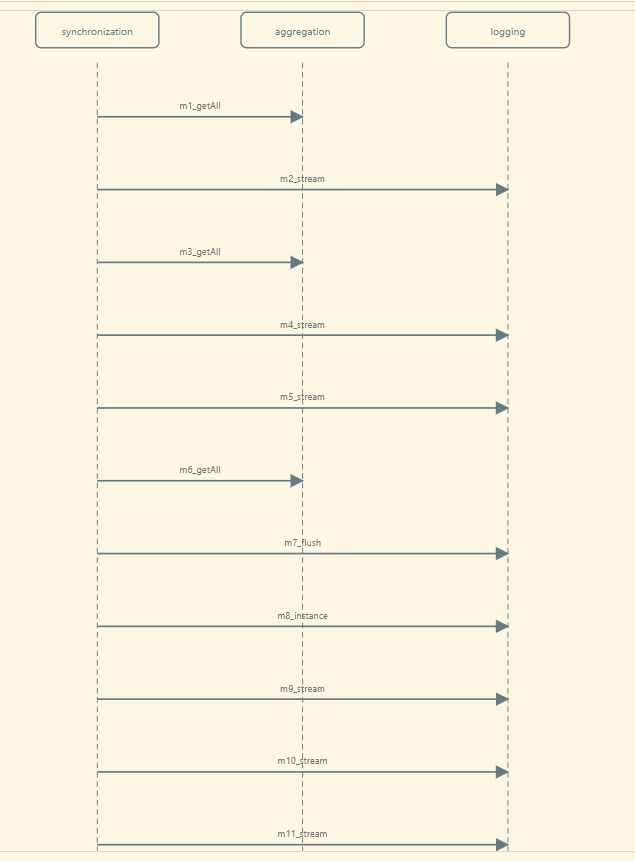
\includegraphics[width=0.85\textwidth]{figures/s1-sequence.png}
\caption{An example of the pipeline's final rendered output: the generated
  \sysml sequence diagram for scenario~S1 (Aggregator notification chain),
  one of the reconstructions evaluated in \cref{sec:h1}. The complete set
  of generated diagrams is reproduced in \cref{sec:appendix-sysmlv2}.}
\label{fig:s1-sequence-main}
\end{figure}

The complete set of generated SysML v2 sequence and structural diagrams
is reproduced in \cref{sec:appendix-sysmlv2}, covering all 14
auto-generated scenarios (Aggregation, Synchronization, IDC, IPC, Redis,
Serial, Signal Handler, Utilities, Data Presentation, and Test Execution
flows).

\section{Scenario Suite and Experimental Conditions}\label{sec:scenario-suite}

The stages above produce the raw artefacts (the static sequence
dependency table and the real \texttt{csp\_matcher} trace log) feeding
the H1 and H2 experiments in \cref{ch:analysis}. This section documents
how those artefacts were assembled into experimental configurations.

\subsection{Scenario Suite (S1--S4)}\label{sec:scenarios}

Four scenarios were defined on CPSCore. The first three (S1--S3) cover
happy-path behaviour across the Aggregation, Synchronization and
Redis/IDC subsystems, occurring naturally in the existing code. S4 is
purpose-built production code, added for a narrow reason: nothing in
S1--S3 could show combining (C4) strictly exceeding both single-source
conditions at once, since CPSCore has no boundary where static and
dynamic evidence each miss a different interaction. S4 introduces one.

\begin{description}
  \item[S1: Aggregator notification chain.]
    \emph{Primary:} Synchronization. \emph{Targets:} Aggregation, Logging.
    The observer/notification pattern:
    \texttt{SynchronizedRunner.runSynchronized}~$\to$~\texttt{Aggregator.getAll},
    followed by logging calls. The \texttt{boost::signals2} callback
    chain is invisible in a static include graph, making this a test of
    IDC topology recovery. \emph{Reference interactions:} 4 (getAll,
    stream, flush, instance).

  \item[S2: Configuration property mapping.]
    \emph{Primary:} Configuration. \emph{Target:} Logging. A mostly-static,
    linear chain: \texttt{PropertyMapper.add}~$\to$~\texttt{RAIILogStream.stream}.
    The easy-case baseline, expected to be reconstructed well even by
    static-only conditions. \emph{Reference interactions:} 1 (stream).

  \item[S3: Multi-component runner orchestration.]
    \emph{Primary:} Synchronization. \emph{Targets:} Aggregation, Utilities,
    Logging. Fan-out from \texttt{SimpleRunner.runStage} to multiple
    independent subsystems at once. The hardest case for static analysis:
    call targets resolved at runtime via template/virtual dispatch produce
    two false-positive static edges (\texttt{flush}, \texttt{instance});
    agentic synthesis (C5) corrects one (\texttt{instance}) but retains
    \texttt{flush} as a disclosed residual imprecision
    (\cref{sec:h1-c5}). \emph{Reference interactions:} 3
    (getAll, stream, convert).

  \item[S4: Stage event pub-sub bridge (constructed).]
    \emph{Primary:} Synchronization. \emph{Targets:} Aggregation, Logging.
    Unlike S1--S3, this is not an existing code path but two new
    production files: \texttt{StageEventBridge} publishes a
    stage-completion event over a \texttt{boost::signals2::signal};
    \texttt{StageEventListener} connects \texttt{onStageEvent} as a slot
    with no static call site anywhere in the codebase. If no listener is
    connected, \texttt{StageEventBridge} logs a \texttt{CPSLOG\_ERROR} to
    \texttt{stream}, suppressed at runtime by a
    \texttt{CPSLogger::LogLevelScope(LogLevel::NONE)} idiom. The
    signal/slot dispatch has no resolvable static call expression, so C2
    sees \texttt{stream} but not \texttt{onStageEvent}, while C3 sees the
    reverse, the one construction in the suite where C2 and C3 each
    miss a different edge rather than one containing the other.
    \emph{Reference interactions:} 2 (stream, onStageEvent).
\end{description}

S4 is marked constructed rather than found-in-the-wild: its ground
truth was authored from the new source files directly, though its
dynamic trace, like S1--S3's, is a real \texttt{csp\_matcher} capture from
running the accompanying Catch2 test under instrumentation; none of
the S1--S4 traces are synthetic. It is reported and stratified
separately from S1--S3 throughout \cref{sec:h1} for this reason, never
folded silently into the happy-path numbers.

Each scenario's ground truth was first drawn by hand from direct source
inspection: the relevant directories, classes and call sites, together
with the test case that exercises them, and only then transcribed into
the \sysml textual reference diagrams used for scoring. \Cref{sec:h1-corrections}
explains why this independence from the pipeline's own output mattered.
Both forms, for all four scenarios, are reproduced in
\cref{sec:appendix-groundtruth}.

\subsection{Five-Condition Design (C1--C5)}\label{sec:conditions}

Each scenario was reconstructed independently under five conditions:

\begin{description}
  \item[C1: LLM-only.] Reconstruction by an \ac{LLM} reasoning over raw
    source code alone, with no access to the static graph or any trace,
    a baseline for what an agent can infer without the pipeline.
  \item[C2: Static-only.] The sequence dependency table extracted from
    \texttt{CppCalls} edges alone (\cref{sec:seq-table}).
  \item[C3: Dynamic-only.] The real runtime trace from \texttt{csp\_matcher}
    instrumentation alone (\cref{sec:trace-impl}).
  \item[C4: Static + Dynamic (combined).] The raw, scenario-scoped union
    of the static and trace artefacts (both already scoped to the
    scenario's declared components at Stage~2, \cref{sec:query-impl}),
    tagged by source but otherwise unpruned.
  \item[C5: Full pipeline.] C4 passed through agentic synthesis
    (\cref{sec:agentic-synthesis,sec:agentic-synthesis-impl}), which
    prunes over-approximated static edges and adjudicates single-source
    interactions by corroboration, suppression and indirect dispatch;
    the complete approach proposed in this thesis.
\end{description}

C1--C4 test \hyperref[sec:h1]{H1} (whether combining sources improves
reconstruction accuracy over any single source); C4 versus C5 shows what
agentic synthesis contributes on top of the raw union, namely pruning
false positives without losing true positives (\cref{sec:h1-results}).
\hyperref[sec:h2]{H2} is tested separately, by the guided-versus-full
instrumentation comparison below (\cref{sec:guided-vs-full}), not by any
pair of the five conditions above.

\subsection{Guided versus Full Instrumentation}\label{sec:guided-vs-full}

H2 requires a second axis, orthogonal to the five conditions above: how
the trace itself is collected.

\begin{description}
  \item[Full instrumentation.] \texttt{csp\_matcher} probes are inserted
    at every candidate call site in the static graph, independent of
    scenario.
  \item[Code-graph-guided instrumentation.] Probes are inserted only at
    call sites within the scenario scope (\cref{sec:scenario-scoping}),
    computed \emph{before} instrumentation rather than filtered after.
\end{description}

This is what makes the H2 comparison meaningful: whether using the code
graph to decide where to look produces a cleaner trace than
instrumenting everything and filtering afterwards, at equivalent or
better coverage. Results (node/edge/noise reduction, coverage) are
reported in \cref{sec:h2-results}.

\begin{table}[htb]
\centering
\caption{Quantitative outcomes per pipeline stage on CPSCore.}
\label{tab:impl-summary}
\begin{tabular}{@{} l r @{}}
\toprule
\textbf{Artefact} & \textbf{Count} \\
\midrule
Graph node labels                            & 11 \\
Graph relationship types                     & 11 \\
Sequence dependency table rows               & 2,574 \\
Unique client$\to$server function pairs (static) & 2,169 \\
Distinct components in sequence table        & 121 \\
Instrumentation targets (functions)          & 9 \\
Source files instrumented                    & 5 \\
Total trace events (csp\_matcher)             & 27 \\
Unique client$\to$server pairs (trace)        & 26 \\
SysML v2 scenarios generated                 & 14 \\
Test assertions passing post-instrumentation & 1,425 / 1,425 \\
\bottomrule
\end{tabular}
\end{table}
